\documentclass{beamer}
\usepackage{listings}
\lstset{
%language=C,
frame=single, 
breaklines=true,
columns=fullflexible
}
\usepackage{subcaption}
\usepackage{setspace}
\usepackage{url}
\usepackage{tikz}
\usepackage{tkz-euclide} % loads  TikZ and tkz-base
%\usetkzobj{all}
\usepackage[utf8]{inputenc}
\usepackage{longtable}
\usetikzlibrary{calc,math}
\usepackage{float}
\usetheme{Berlin}
\usepackage{graphicx}
\usepackage{hyperref}
\usecolortheme{beaver}


\newcommand\norm[1]{\left\lVert#1\right\rVert}
\renewcommand{\vec}[1]{\mathbf{#1}}
\usepackage[export]{adjustbox}
\usepackage[utf8]{inputenc}
\usepackage{amsmath}
%\usetheme{Boadilla}
\newcommand\mytextbullet{\leavevmode%
\usebeamertemplate{itemize item}\hspace{.5em}}

\bibliographystyle{IEEEtran}

\usepackage{color}

\title{7-Segment Display using VAMAN}
\author{B603 Lab}
%{\and} \\
%\vspace{10pt}
%{Supervisor:} \\
%{Dr. GVV Sharma} }

\institute{Indian Institute of Technology, Hyderabad.}
\date{\today}

\begin{document}


\begin{frame}
\titlepage
\end{frame}


\section{Components}
\begin{frame}
\frametitle{Components}
\begin{columns}
\column{1\textwidth}
  \begin{enumerate}
  \item Vaman
  \vspace{10pt}
  \item 7447 IC
  \vspace{10pt}
  \item 7 Segment Display
  
  
  \end{enumerate}
  
\end{columns}

\end{frame}

\section{Pinout Diagram of 7-Segment Display}
\begin{frame}
\frametitle{Pinout Diagram of 7-Segment Display}
\begin{columns}
\column{1\textwidth}
\begin{figure}[h!]
  \centering
  \begin{subfigure}[b]{0.75\linewidth}
    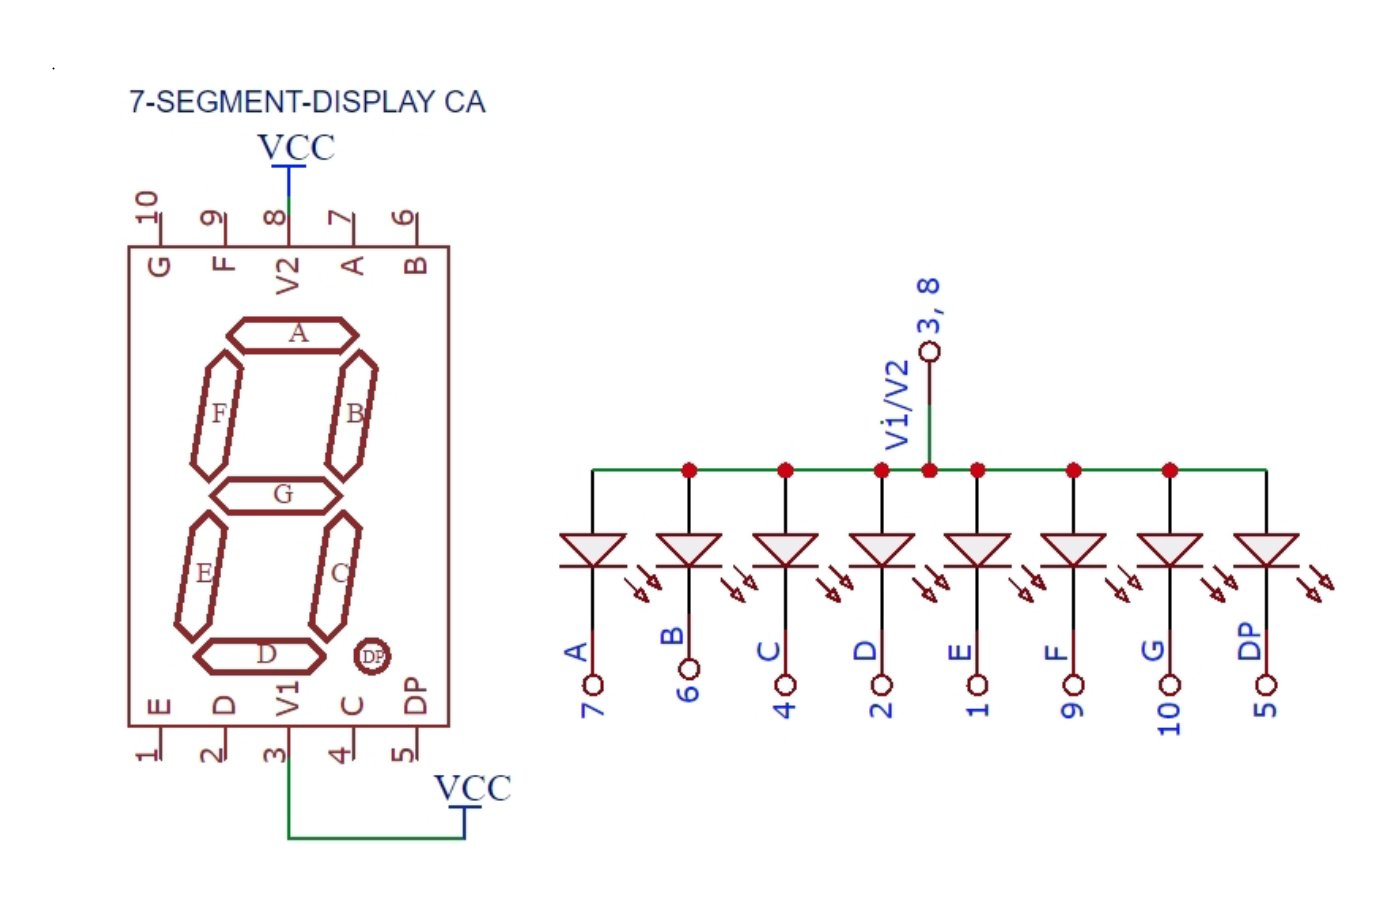
\includegraphics[width=\linewidth]{seven_segment.jpg}
%    \caption{Coffee.}
  \end{subfigure}

 % \caption{Flysky Receiver}
%  \label{fig:axis}
\end{figure}



%\caption{Flysky Receiver}
  
\end{columns}
%\vspace{25px}



\end{frame}

\section{Flow Chart }
\begin{frame}
\frametitle{Flow Chart: }
\begin{figure}[h!]
  \centering
  \begin{subfigure}[b]{0.75\linewidth}
    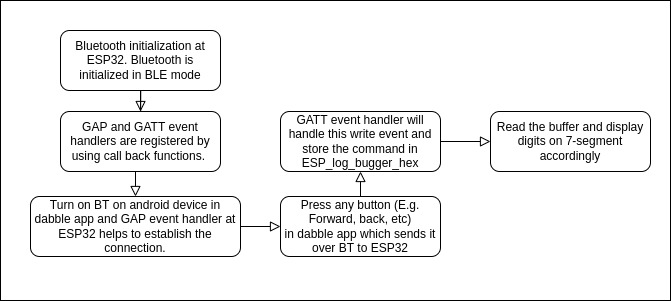
\includegraphics[width=\linewidth]{flowdiag_vaman .jpg}
%    \caption{Coffee.}
  \end{subfigure}


\end{figure}




\end{frame}

\section{Wiring Diagram:}
\begin{frame}
\frametitle{Wiring Diagram:}

\begin{figure}[h!]
  \centering
  \begin{subfigure}[b]{0.75\linewidth}
    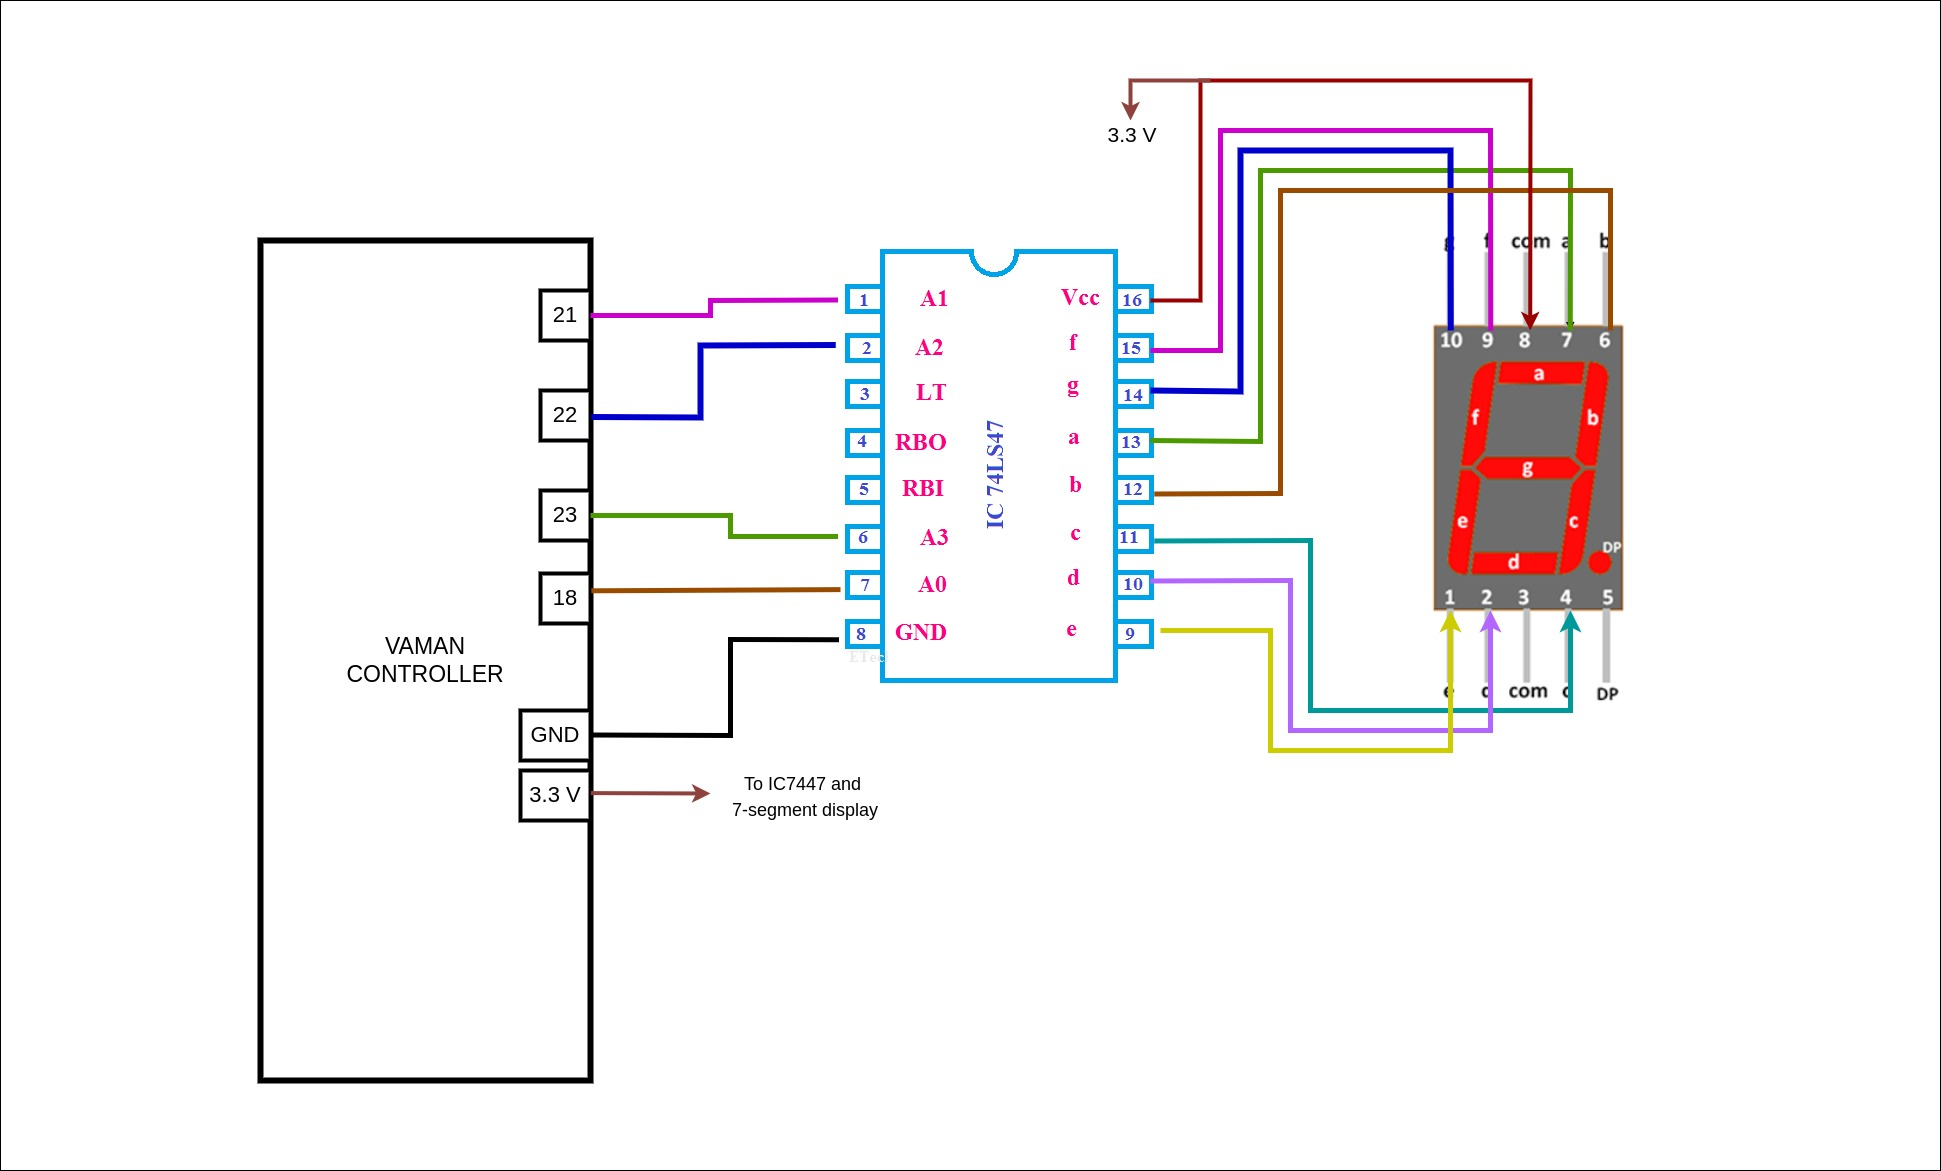
\includegraphics[width=\linewidth]{Wiring.jpg}
%    \caption{Coffee.}
  \end{subfigure}


\end{figure}

\end{frame}



\section{Code}
\begin{frame}
\frametitle{Code}
\begin{columns}
\column{1\textwidth}

  \begin{itemize}
  \item  Flash the code to Vaman.\\
  \url{https://github.com/AnilMondedla/Vaman/blob/main/Vaman_spi/main/hello_world_main.c}
  
  
  \end{itemize}
  \  
\end{columns}
%\vspace{25px}



\end{frame}
\end{document}















